\section{拉伸建模法}
\subsection{绘制垫片主视图}\label{sec:dianpian}
\begin{procedure}
\item 设置图层。

图\ref{fig:tiaoyafadianpian}中不仅有实线还有中心线。中心线是用于表达图对称中心位置的图线。为方便对各类图线进行统一管理,需要应用AutoCAD的图层管理。所谓图层就是将属性相同的对象绘制在一张类似于透明的纸上,将不同属性的对象绘制在不同的透明纸上,以实现图形对象的分类管理,最后将所有的透明纸叠加在一起就构成了整个图形。设置【图层】的方法有:
\begin{itemize}
\item 键盘输入LAYER\index{layer}或LA。
\item 【格式】$\rightarrow$【图层】。
\item 【工具栏】$\triangleright$【图层】图标
\includegraphics[scale=0.6]{layertool.png}。
\end{itemize}
以上三种方法都将启动图\ref{fig:layerdialog}所示的【图层特性管理器】对话框。
\begin{figure}[htbp]
\centering
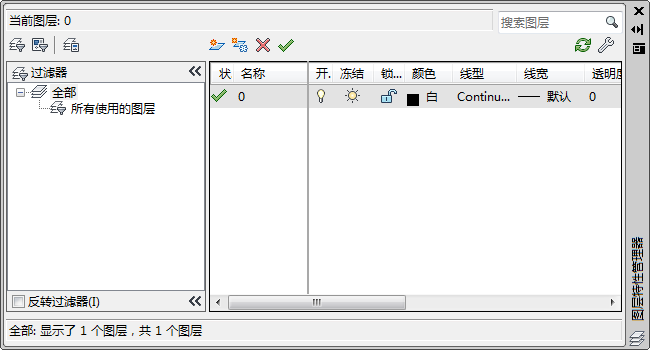
\includegraphics[scale=0.4]{layerdialog.png}
\caption{【图层特性管理器】对话框}\label{fig:layerdialog}
\end{figure}

单击【图层特性管理器】对话框中的【新建图层】图标
\includegraphics[scale=0.6]{newlayer.png},新建中心线图层和实线图层,分别取名为“中心线”和“实线”。

\begin{figure}[htbp]
\centering
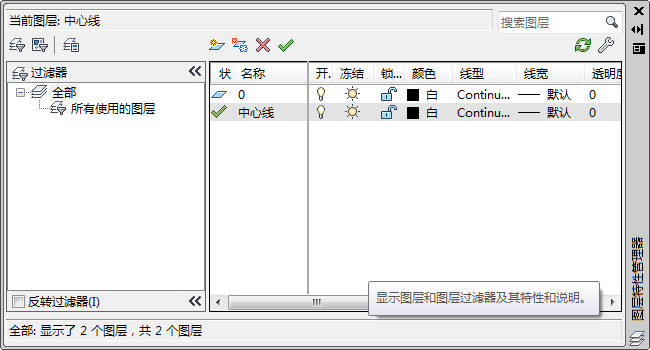
\includegraphics[scale=0.4]{layersetresult1.png}
\caption{新建图层结果}\label{fig:layersetresult1}
\end{figure}

选中新建的“中心线”图层,单击【置为当前】图标
\includegraphics[scale=0.6]{setcurrentlayer.png},即可将“中心线”图层置为当前,结果如图\ref{fig:layersetresult1}所示。

为便于区分各图层的对象,需要设置各图层的颜色。为此我们将实线图层的颜色设置为红色,将中心线图层设置为蓝色。具体设置方法是:单击“实线”图层
\includegraphics[scale=0.5]{solidlayerset.png}中的
\includegraphics[scale=0.6]{coloricon.png}图标,弹出如图\ref{fig:colorselect}所示的【选择颜色】对话框,选择红色颜色,并单击【确定】。“中心线”层的设置方法与“实线”层的设置方法相同。

\begin{figure}[htbp]
\centering
\begin{floatrow}
\ffigbox{\caption{【选择颜色】对话框}\label{fig:colorselect}}{
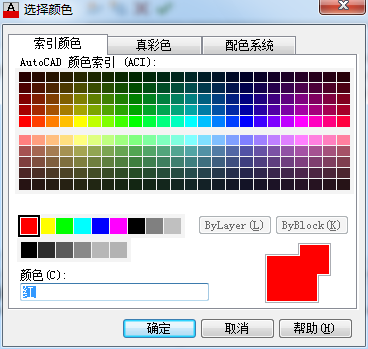
\includegraphics[scale=0.37]{colorselect.png}
}
\ffigbox{\caption{【线宽】对话框}\label{fig:linewidthselect}}{

\includegraphics[scale=0.4]{linewidthselect.png}
}
\end{floatrow}
\end{figure}

接下来设置实线层的线宽,单击实线层中的线宽图标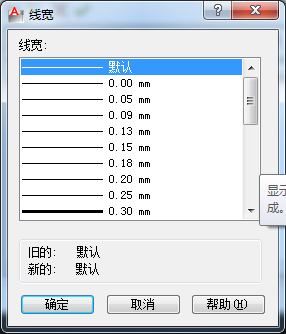
\includegraphics[scale=0.6]{linewidthset.png},弹出如图\ref{fig:linewidthselect}所示的【线宽】对话框,选择0.7mm的线宽作为实线层的线宽,单击确定。

接下来,将中心线图层的线型设置为CENTER图线。具体设置方法为:单击“中心线”层中的线型名
\includegraphics[scale=0.6]{linetypeicon.png}l图标,弹出如图\ref{fig:linetypeset}所示的【选择线型】对话框。此时还没我所需要的线型,需要单击对话框中的【加载...】按钮,弹出如图\ref{fig:loadlinetype}所示的【加载或重载线型】对话框,选择CENTER图线并确定,完成线型加载。最后在【选择线型】对话框中选中新加载的CENTER图线,再一次单击确定,完成线型的设置。
\begin{figure}[htbp]
\centering
\begin{floatrow}
\ffigbox{\caption{【选择线型】对话框}\label{fig:linetypeset}}{
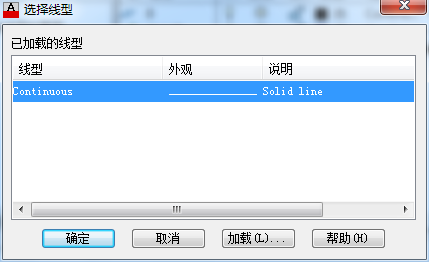
\includegraphics[scale=0.4]{linetypeset.png}
}
\ffigbox{\caption{【加载或重载线型】对话框}\label{fig:loadlinetype}}{
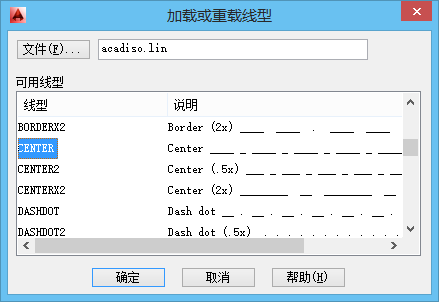
\includegraphics[scale=0.33]{loadlinetype.png}
}
\end{floatrow}
\end{figure}

完成上述操作后,我们会得到图\ref{fig:layersetresult2}所示图层设置结果。完成设置后单击对话框中的关闭按钮退出图层设置,返回绘图界面。
\begin{figure}[htbp]
\centering
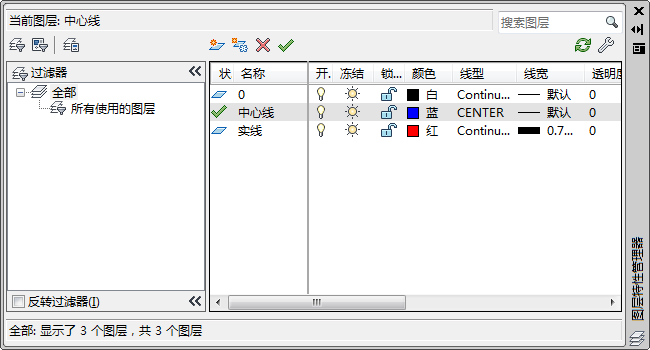
\includegraphics[scale=0.4]{layersetresult2.png}
\caption{图层设置结果}\label{fig:layersetresult2}
\end{figure}

\item 切换视图为主视图。
\item 绘制中心线,其结果如图\ref{fig:centerresult}所示。

用【构造线】命令绘制出对称中心线。【构造线】命令的启动方法有:
\begin{itemize}
\item 键盘输入XLINE\index{xline}或XL。
\item 【绘图】$\rightarrow$【构造线】。
\item 【绘图】$\triangleright$【构造线】图标
\includegraphics[scale=0.6]{xlinetool.png}。
\end{itemize}
\begin{lstlisting}
|命令: XLINE|
|指定点或 [水平(H)/垂直(V)/角度(A)/二等分(B)/偏移(O)]: 52,52|
|指定通过点:$ @1<0$|
|指定通过点:$ @1<90$|
|指定通过点:|
\end{lstlisting}

用CIRCLE命令绘制$\diameter 84$的中心线圆。
\begin{lstlisting}
|命令: CIRCLE|
|指定圆的圆心或 [三点(3P)/两点(2P)/切点、切点、半径(T)]:INT|
|指定圆的半径或 [直径(D)]: 42|
\end{lstlisting}
\item 切换图层为“实线”层。切换图层的方法有:
\begin{itemize}
\item 在【工具栏】中点击
\includegraphics[scale=0.6]{layercontral.png}图标,从弹出的列表中选择“实线”项,即可完成图层的切换。
\item 用【图层特性管理器】将“实线”层设置为当前。
\end{itemize}
\item 绘制圆。

用对称中心线的交点作$\diameter 104$、$\diameter 53$和$\diameter 8$的圆,其结果如图\ref{fig:dianpiancircle}所示。

首先绘制$\diameter 104$的圆。
\begin{lstlisting}
|命令: circle|
|指定圆的圆心或 [三点(3P)/两点(2P)/切点、切点、半径(T)]:int|
|指定圆的半径或 [直径(D)] $<42.0000>$: 52|
\end{lstlisting}
将图层切换为“实线”图层,再绘制$\diameter 53$的圆。
\begin{lstlisting}
|命令: circle|
|指定圆的圆心或 [三点(3P)/两点(2P)/切点、切点、半径(T)]:|
|指定圆的半径或 [直径(D)]$ <52.0000>$: 26.5|
\end{lstlisting}
最后绘$\diameter 8$的圆。
\begin{lstlisting}
|命令: circle|
|指定圆的圆心或 [三点(3P)/两点(2P)/切点、切点、半径(T)]:|
|指定圆的半径或 [直径(D)] $<26.5000>$: 4|
\end{lstlisting}

\begin{figure}[htbp]
\centering
\subfloat[]{\label{fig:centerresult}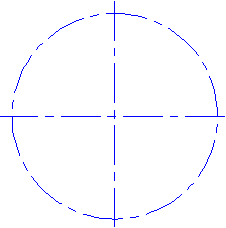
\includegraphics[scale=0.8]{centerresult.png}}\hspace{20pt}
\subfloat[]{\label{fig:dianpiancircle}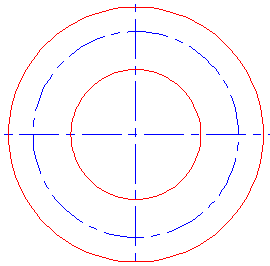
\includegraphics[scale=0.7]{dianpiancircle.png}}
\caption{绘制中心线和圆}
\end{figure}
\item 阵列圆。环形阵列的启动方法有:
\begin{itemize}
\item 键盘输入ARRAYPLOAY\index{arrayploay}。
\item 【修改】$\rightarrow$【阵列】$\rightarrow$【环形阵列】。
\item 【修改】$\triangleright$【环形阵列】图标
\includegraphics[scale=0.6]{arrayploaytool.png}。
\end{itemize}

\begin{figure}[htbp]
\centering
\subfloat[]{\label{fig:arraypolayselect}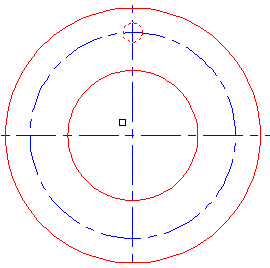
\includegraphics[scale=0.5]{arraypolayselect.png}}\hspace{20pt}
\subfloat[]{\label{fig:arraypolaycenter}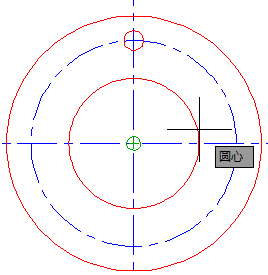
\includegraphics[scale=0.5]{arraypolaycenter.png}}\hspace{20pt}
\subfloat[]{\label{fig:arraypolayresult}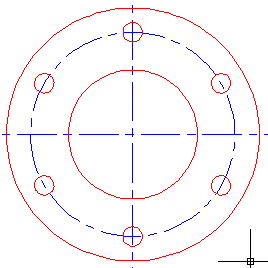
\includegraphics[scale=0.5]{arraypolayresult.png}}
\caption{环形阵列过程}
\end{figure}

启动阵列后要求选择需要阵列的对象,选择图\ref{fig:arraypolayselect}所示的$\diameter 8$圆做为要阵列的对象,并结束对象选择。
\begin{lstlisting}
|命令: ARRAYPOLAR|
|选择对象: 找到 1 个|
|选择对象:|
|类型 = 极轴  关联 = 是|
\end{lstlisting}
接下来指定阵列中,以图\ref{fig:arraypolaycenter}所示的方式选择圆心作为阵列的中心点。
\begin{lstlisting}
|指定阵列的中心点或 [基点(B)/旋转轴(A)]:|
\end{lstlisting}
默认情况下将产生图\ref{fig:arraypolayresult}所示的由6个圆组成的环形阵列。若要产生其它数目的环形阵列,则需要使用【项目(i)】选项,并指定阵列数;若要产生非360度填充角度,则需要使用【填充角度(F)】选项,并指定填充角度。
\begin{lstlisting}
|选择夹点以编辑阵列或 [关联(AS)/基点(B)/项目(I)/项目间角度(A)/填|
|充角度(F)/行(ROW)/层(L)/旋转项目(ROT)/退出(X)] $<$退出$>$:|
\end{lstlisting}
\end{procedure}
\endinput